\documentclass[14pt]{beamer}
\usepackage{luatexja-fontspec}
\newjfontface{\nonproportional}{BIZ UDMincho}[YokoFeatures={JFM=ujis}]
\setmainjfont[Ligatures={Common,TeX},
  ItalicFont={BIZ UDPMincho},
  ItalicFeatures={FakeSlant=0.27},
  SlantedFont={BIZ UDPMincho},
  SlantedFeatures={FakeSlant=0.18},
  BoldFont={BIZ UDPGothic Bold},
  BoldSlantedFont={BIZ UDPGothic Bold},
  BoldSlantedFeatures={FakeSlant=0.18},
  BoldItalicFont={BIZ UDPGothic Bold},
  BoldItalicFeatures={FakeSlant=0.27},
  YokoFeatures={JFM=prop}]{BIZ UDPMincho}
%\newjfontface{\nonproportional}{BIZ UDGothic}[YokoFeatures={JFM=ujis}]
\setsansjfont[Ligatures={Common,TeX},
  ItalicFont={BIZ UDPGothic},
  ItalicFeatures={FakeSlant=0.23},
  SlantedFont={BIZ UDPGothic},
  SlantedFeatures={FakeSlant=0.23},
  BoldFont={BIZ UDPGothic Bold},
  BoldSlantedFont={BIZ UDPGothic Bold},
  BoldSlantedFeatures={FakeSlant=0.23},
  BoldItalicFont={BIZ UDPGothic Bold},
  BoldItalicFeatures={FakeSlant=0.23},
  YokoFeatures={JFM=prop}]{BIZ UDPGothic}
\usepackage{beamerthemesplit}
\usepackage{caption}
\captionsetup[figure]{labelformat=empty,labelsep=none}
\usepackage{svg}
\usepackage[]{graphicx}
\svgsetup{
  inkscapelatex=false
}

\usepackage{listings,jvlisting}
\lstset{
  language=C++,
  basicstyle=\ttfamily\footnotesize,
  % keywordstyle=\bfseries\color{green},
  showstringspaces=false,
  frame={tb},
  %numbers=left,
  xrightmargin=0\zw,
  xleftmargin=0\zw,
  % columns=[l]{fullflexible},
  columns=fixed,
  basewidth=0.5em,
  numberstyle = \footnotesize,
  frame = tbrl,
  captionpos = b,
  moredelim=[is][\color{green}\bfseries]{<\#green\#}{\#>},
  moredelim=[is][\color{blue}\bfseries]{<\#blue\#}{\#>},
  moredelim=[is][\color{red}\bfseries]{<\#red\#}{\#>},
  moredelim=[is][\color{yellow}\bfseries]{<\#yellow\#}{\#>},
  moredelim=[is][\color{magenta}\bfseries]{<\#magenta\#}{\#>},
}

\usetheme{Boadilla}
%Beamerフォント設定
\usefonttheme{professionalfonts} % Be professional!
\usepackage[T1]{fontenc}
%\usepackage{mlmodern}  % 太いComputer Modern
%\usepackage{newtxtext} % 数式以外をTXフォントで上書き
%\usepackage[deluxe,uplatex]{otf} % 日本語多ウェイト化
\renewcommand{\familydefault}{\sfdefault}  % 英文をサンセリフ体に
\renewcommand{\kanjifamilydefault}{\gtdefault}  % 日本語をゴシック体に
\usefonttheme{structurebold} % タイトル部を太字
\setbeamerfont{alerted text}{series=\bfseries} % Alertを太字
\setbeamerfont{section in toc}{series=\mdseries} % 目次は太字にしない
\setbeamerfont{frametitle}{size=\Large} % フレームタイトル文字サイズ
\setbeamerfont{title}{size=\LARGE} % タイトル文字サイズ
\setbeamerfont{date}{size=\small}  % 日付文字サイズ
%Beamer色設定
\definecolor{UniBlue}{RGB}{0,150,200}
\definecolor{AlertOrange}{RGB}{255,76,0}
\definecolor{AlmostBlack}{RGB}{38,38,38}
\setbeamercolor{normal text}{fg=AlmostBlack}  % 本文カラー
\setbeamercolor{structure}{fg=UniBlue} % 見出しカラー
\setbeamercolor{block title}{fg=UniBlue!50!black} % ブロック部分タイトルカラー
\setbeamercolor{alerted text}{fg=AlertOrange} % \alert 文字カラー
\mode<beamer>{
    \definecolor{BackGroundGray}{RGB}{254,254,254}
    \setbeamercolor{background canvas}{bg=BackGroundGray} % スライドモードのみ背景をわずかにグレーにする
}
%フラットデザイン化
\setbeamertemplate{blocks}[rounded] % Blockの影を消す
\useinnertheme{circles} % 箇条書きをシンプルに
\setbeamertemplate{navigation symbols}{} % ナビゲーションシンボルを消す
\setbeamertemplate{footline}[frame number] % フッターはスライド番号のみ

\usepackage{tikz}
\usepackage[absolute,overlay]{textpos}

\usepackage{pxrubrica} %ルビ

%教科書対応ページのマクロ
\newcommand{\textpageref}[1]{{
  \begin{textblock*}{0.4\linewidth}(285pt,5pt)
    \begin{tikzpicture}
        \node[rectangle,fill=cyan!10,text width=2.3cm, text centered,rounded corners]{教科書\\{#1}ページ};
    \end{tikzpicture}
  \end{textblock*}
}}

% 余白を広げる
\setbeamersize{text margin left=15pt, text margin right=15pt}
\setbeamertemplate{footline}[frame number]
\title{子どもIT未来塾 第7回}
\author{奥山 祐市}

\begin{document}

\frame{
   \begin{center}
    \huge{子どもIT未来塾 第7回}\\

    \vspace{34pt}
	   {\huge 音声合成と音声認識}\\
    \vspace{24pt}
    \large{奥山 祐市}\\
    \vspace{10pt}
    \large{2026年9月26日}
  \end{center}
}

\begin{frame}[fragile]
    \frametitle{使うファイルをコピーしよう}
    \begin{itemize}
        \item 下のコマンドを実行しよう
        \item 「\textasciitilde(チルダ)」記号とスペースに気をつけよう
    \end{itemize}
    \begin{lstlisting}[title=使うファイルのコピー,label=workfilecopy-part1]
<#green#pi@raspberrypi#>:<#blue#~ $#> cp -r /usr/local/share/ome/07 ~/07/
<#green#pi@raspberrypi#>:<#blue#~ $#>
    \end{lstlisting}
    \textpageref{1}
\end{frame}

\begin{frame}
	\frametitle{今日やること}
  \begin{enumerate}
    \item 音声合成
    \begin{enumerate}
      \item 音声合成とは
      \item Open JTalkとは
    \end{enumerate}
    \item 音声認識
    \begin{enumerate}
      \item 音声認識とは
      \item Juliusとは
    \end{enumerate}
  \end{enumerate}
\end{frame}

\begin{frame}
  \frametitle{音声合成}
  \vspace{30pt}
  \begin{center}
  人間の音声を人工的に作りだすこと
  \begin{figure}
    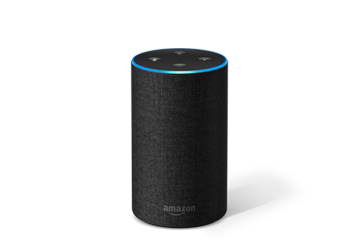
\includegraphics[width=.5\textwidth]{../asset/image/amazon_echo.png}
    \caption{Amazon Echo（出典：Amazon.com, Inc）}
  \end{figure}
  \end{center}
  \textpageref{2}
\end{frame}

\begin{frame}
  \frametitle{Open JTalk}
  \begin{itemize}
    \item 音声合成のためのソフトウェア
    \item 文章と声の特徴データから音声を作る
  \end{itemize}
  \begin{center}
  \includesvg[width=0.8\textwidth]{../asset/image/text06-img011.svg}
  \end{center}
  \textpageref{2}
\end{frame}

\begin{frame}
  \frametitle{音声認識}
  \vspace{20pt}
  \begin{itemize}
    \item 人が話した声を文字に変えること
    \item 話し言葉から文字列への変換
  \end{itemize}
  \begin{center}
  \begin{figure}[tbp]
  \begin{minipage}[b]{0.45\columnwidth}
    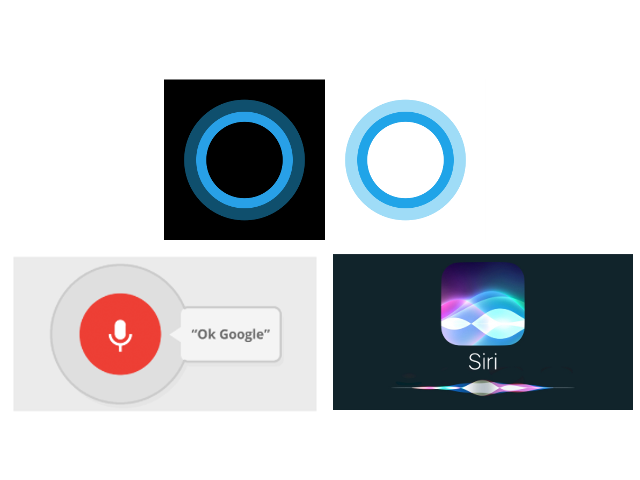
\includegraphics[width=\columnwidth]{../asset/image/voice_assistant.png}
    \caption{\scriptsize 携帯、スマートフォン、コンピュータの音声認識アシスタント}
  \end{minipage}
  \hspace{0.04\columnwidth}
  \begin{minipage}[b]{0.3\columnwidth}
    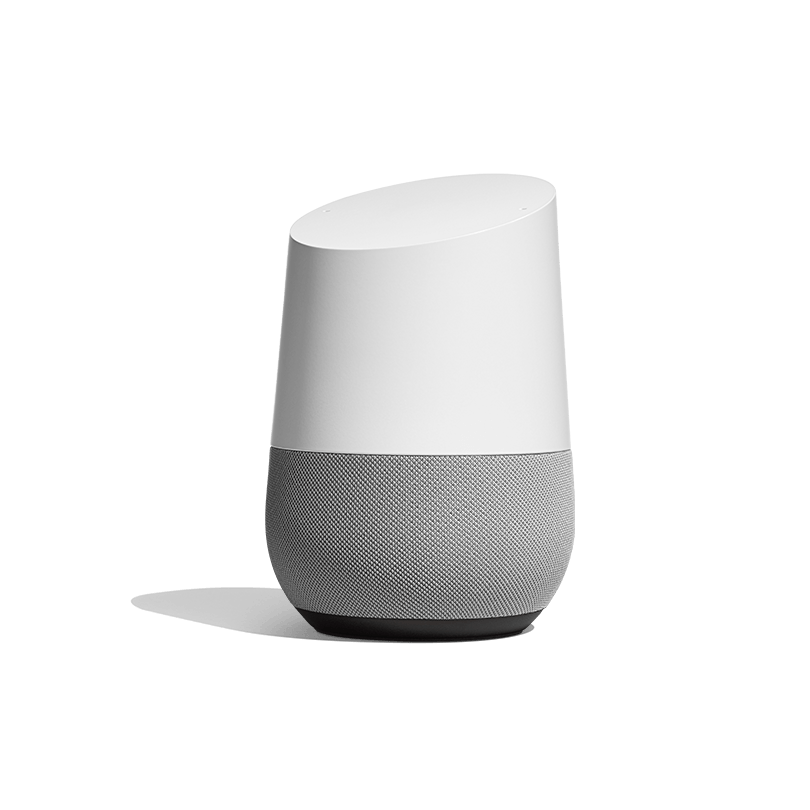
\includegraphics[width=\columnwidth]{../asset/image/google_home.png}
    \caption{\scriptsize Google Home}
  \end{minipage}
  \end{figure}
  \end{center}
  \textpageref{3}
\end{frame}

\begin{frame}
  \frametitle{Julius}
  \begin{itemize}
    \item 音声認識のためのソフトウェア
    \item 音声を聞き取って文字に変換する
  \end{itemize}
  \begin{center}
  \includesvg[width=0.8\textwidth]{../asset/image/Julius.svg}
  \end{center}
  \textpageref{3}
\end{frame}

\begin{frame}
  \begin{exampleblock}{問題を解いてみよう}
    \begin{itemize}
      \item 教科書3ページ 問題7-1(2問)
      \item 教科書3ページ 問題7-2(1問)
    \end{itemize}
  \end{exampleblock}
  \textpageref{3}
\end{frame}

\begin{frame}
  \centering
  {\Large 準備}
\end{frame}

\begin{frame}
  \frametitle{ヘッドフォンをつけよう}
  電源を入れる前にヘッドセットを接続しよう。
  \begin{center}
  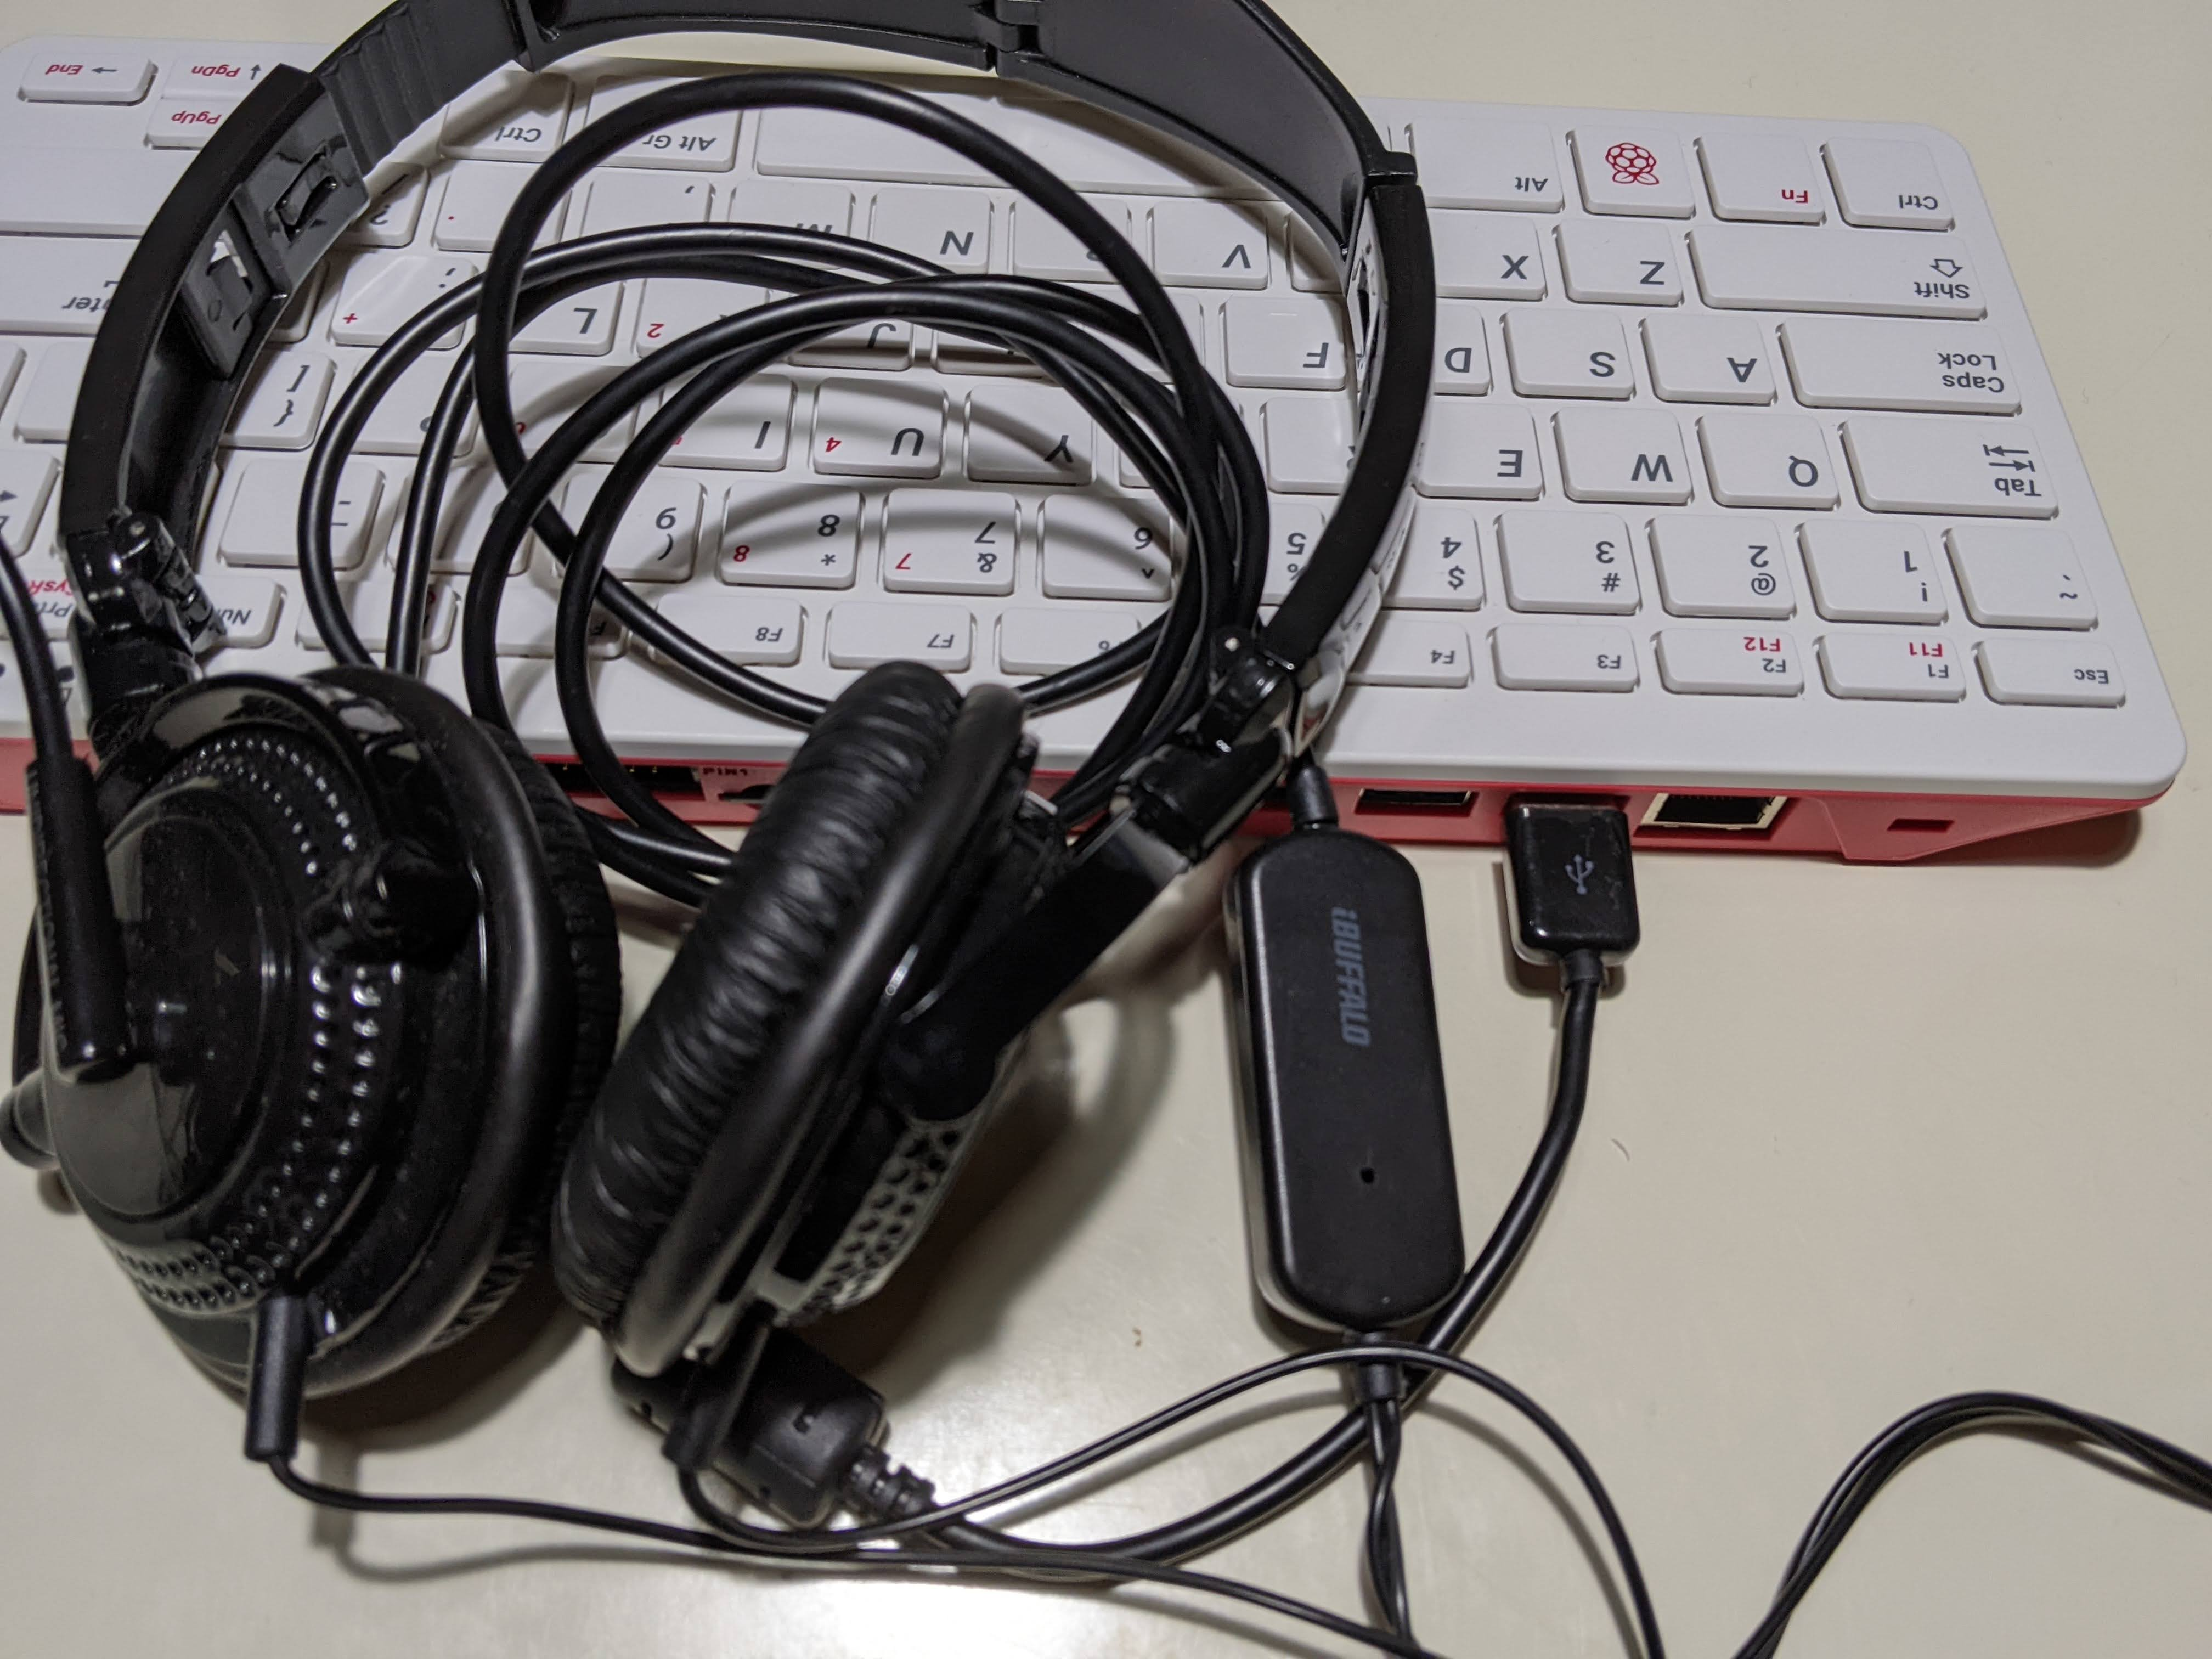
\includegraphics[width=0.65\textwidth]{../asset/image/how_to_connect_headset.jpg}
  \end{center}
  \textpageref{4}
\end{frame}

\begin{frame}
  \frametitle{音声出力の選択}
  \begin{itemize}
    \item スピーカーアイコンを右クリック
    \item USB PnP Sound Deviceを選ぶ
  \end{itemize}
\begin{center}
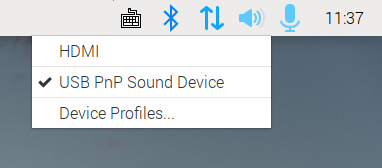
\includegraphics[width=0.6\textwidth]{../asset/image/select_sink.png}
\end{center}
  \textpageref{4}
\end{frame}

\begin{frame}
  \frametitle{マイクミュートについて}

  \begin{itemize}
    \item ヘッドセットのコントローラに赤いランプが点いていると「マイクミュート」
    \item マイクを使うときはマイクミュートを解除しておこう
  \end{itemize}
  \begin{center}
  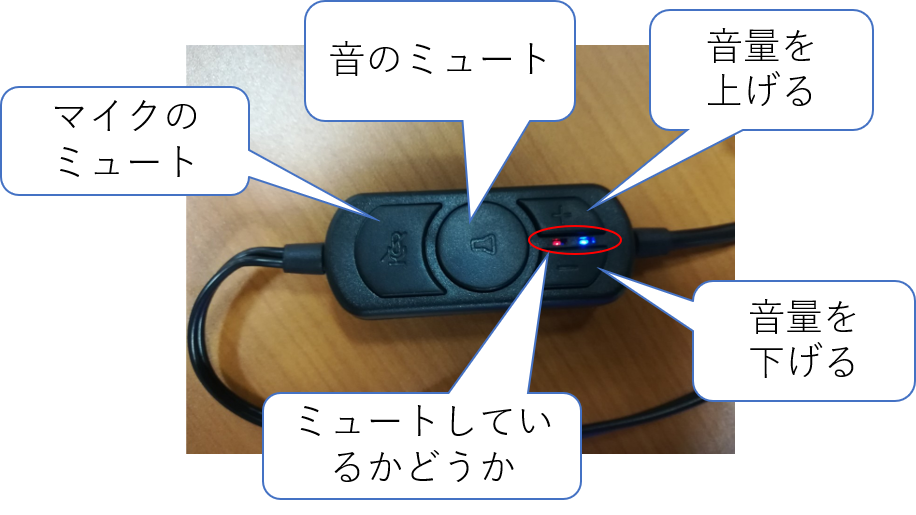
\includegraphics[width=0.65\textwidth]{../asset/image/text06-img004.png}
  \end{center}
  \textpageref{5}
\end{frame}

\begin{frame}
  \frametitle{マイク音量の設定}
  \begin{itemize}
    \item マイクアイコンを左クリック
    \item 教室では入力音量を最大にする
  \end{itemize}
\begin{center}
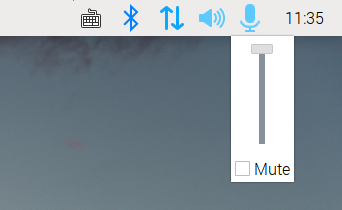
\includegraphics[width=0.65\textwidth]{../asset/image/microphone_volume.png}
\end{center}
  \textpageref{5}
\end{frame}

\begin{frame}
  \frametitle{困ったとき：マイクの復旧}
  \begin{itemize}
    \item マイクアイコンは音量調整のときだけ左クリック
    \item 右クリックのUSB PnP Sound Deviceは押さない
    \item 使えなくなったら、スピーカーを右クリック\\「デバイスプロファイル…」を開く
    \item USBの「アナログステレオ 出力」を選ぶ\\すでに選ばれていたら、一度「オフ」を選ぶ
    \item 「アナログステレオ 出力 + モノ 入力」\\を選んで「OK」
  \end{itemize}
  \textpageref{6～7}
\end{frame}

\begin{frame}
  \centering
  {\Large Open JTalk}
\end{frame}

\begin{frame}[fragile]
  \frametitle{文章を読み上げてもらう -1}

  \begin{lstlisting}[title=\textasciitilde/07/openjtalk.hsp,label=openjtalk.hsp-part1]
  #include "hsp3dish.as"
  #include "jtalk.as"

  redraw 0
  mes "発話開始"
  mes "「子どもIT未来塾」"
  redraw 1

  <#red#jtload "子どもIT未来塾", 0	;音声ファイルを出力し、読み込む#>
  mmplay 0			<#blue#;音声ファイルを再生する#>
  stop
  \end{lstlisting}
  \textpageref{8}
\end{frame}

\begin{frame}
  \frametitle{文章を読み上げてもらう -2}
  \begin{itemize}
    \item プログラムの中の jtload "子どもIT未来塾", 0 の部分を見てみよう
    \item jtload "読ませたい文字列", <バッファ番号>
    \item ""の中の文字列を変えると、好きな言葉を読ませられるよ！
  \end{itemize}
  \textpageref{8}
\end{frame}

\begin{frame}
  \frametitle{問題7-3を解いてみよう}
\begin{exampleblock}{教科書9ページ 問題7-3（2問）}
  \begin{itemize}
    \item 「本日は晴天なり」と読むように変更し、\\sunny.hspとして07フォルダに保存・実行しよう
    \item 時間があれば、好きな言葉を読み上げさせよう
  \end{itemize}
\end{exampleblock}
  \textpageref{9}
\end{frame}

\begin{frame}[fragile]
  \frametitle{声音を変えてみる -1}
  \begin{lstlisting}[title=\textasciitilde/07/voice.hsp,label=voice.hsp-part1]
  #include "hsp3dish.as"
  #include "jtalk.as"

  redraw 0
  mes "発話開始"
  mes "「子どもIT未来塾」"
  redraw 1

  <#red#setvoice "htsvoice-tohoku-f01/tohoku-f01-sad.htsvoice" #>
                             <#red#;声音ファイルを指定#>
  jtload "子どもIT未来塾", 0	<#blue#;音声ファイルを出力し、読み込む#>
  mmplay 0			<#blue#;音声ファイルを再生する#>
  stop
  \end{lstlisting}
  \textpageref{10}
\end{frame}

\begin{frame}
  \frametitle{声音を変えてみる -2}
  \begin{itemize}
    \item 声音（こわね）は、声の種類や話し方のこと
    \item setvoiceで.htsvoiceファイルを指定する
    \item voice.hspと同じ07フォルダの中にある\\htsvoice-tohoku-f01からファイルを探す
    \item 普通・怒った・うれしい・悲しい声を試そう
  \end{itemize}
  \textpageref{10}
\end{frame}

\begin{frame}
  \frametitle{問題7-4を解いてみよう}
\begin{exampleblock}{教科書11ページ 問題7-4（2問）}
  \begin{itemize}
    \item voice.hspを実行してみよう
    \item 時間があれば、好きな声音を使ってみよう
  \end{itemize}
\end{exampleblock}
  \textpageref{11}
\end{frame}

\begin{frame}[fragile]
  \frametitle{日付を読み上げる -1}
  \begin{lstlisting}[title=\textasciitilde/07/readdate.hsp,label=readdate.hsp-part1,basewidth=0.45em]
  #include "hsp3dish.as"
  #include "jtalk.as"

<#red#date = "" + gettime(0) + "年" + gettime(1) + "月" + gettime(3) + "日"#>

    redraw 0
    mes "日付を読み上げます"
    mes date
    redraw 1

    jtload date, 0 <#blue#;dateの文字列から音声を作り、読み込む#>
    mmplay 0 <#blue#;音声ファイルを再生する#>
    stop
  \end{lstlisting}
  \textpageref{12}
\end{frame}

\begin{frame}
  \frametitle{日付を読み上げる -2}
  \begin{itemize}
    \item Open JTalkはdate変数の文字列を読む
    \item gettime(0)：年、(1)：月、(3)：日
    \item gettime(2)：曜日を表す0～6の数\\0=日、1=月、2=火、…、6=土（曜日名ではない）
    \item gettime(4)：時、(5)：分、(6)：秒、(7)：ミリ秒
  \end{itemize}
  \textpageref{12}
\end{frame}

\begin{frame}
  \frametitle{問題7-5を解いてみよう}
\begin{exampleblock}{教科書13ページ 問題7-5（2問）}
  \begin{itemize}
    \item readdate.hspを実行してみよう
    \item 時間があれば、時刻を読み上げるように変えよう
  \end{itemize}
\end{exampleblock}
  \textpageref{13}
\end{frame}

\begin{frame}[fragile]
  \frametitle{計算結果を読み上げる -1}
  \begin{lstlisting}[title=\textasciitilde/07/readcalc.hsp,label=readcalc.hsp-part1]
    #include "hsp3dish.as"
    #include "jtalk.as"
    a = 3
    b = 2

    <#blue#;問題描画#>
    redraw 0
    mes "" + a + " + " + b
    redraw 1

    <#blue#;問題読み上げ#>
    jtload "" + a + "たす" + b, 0
    mmplay 0
    <#red#wait 100#>
  \end{lstlisting}
  \textpageref{14}
\end{frame}

\begin{frame}[fragile]
  \frametitle{計算結果を読み上げる -2}
  \begin{lstlisting}[title=\textasciitilde/07/readcalc.hsp,label=readcalc.hsp-part2]
    <#blue#;答え計算#>
    kotae = a + b

    <#red#;答え読み上げ
    jtload "こたえは" + kotae, 1
    mmplay 1#>
    <#blue#;答え描画#>
    redraw 0
    mes "" + a + " + " + b
    mes "= " + kotae
    redraw 1

    wait 30
    stop
  \end{lstlisting}
  \textpageref{14}
\end{frame}

\begin{frame}
  \frametitle{計算結果を読み上げる -3}
  \begin{itemize}
    \item a + bの計算結果をkotaeに代入する
    \item Open JTalkで問題と答えを読み上げる
    \item wait 100は約1秒待つ命令\\音声が終わったかを自動で判定するわけではない
    \item 長い文章を読むときは待つ時間も長くしよう
  \end{itemize}
  \textpageref{14}
\end{frame}

\begin{frame}
  \frametitle{問題7-6を解いてみよう}
\begin{exampleblock}{教科書15ページ 問題7-6（2問）}
  \begin{itemize}
    \item readcalc.hspを実行してみよう
    \item 時間があれば、引き算の答えを読み上げよう
  \end{itemize}
\end{exampleblock}
  \textpageref{15}
\end{frame}

\begin{frame}
  \centering
  {\Large Julius}
\end{frame}

\begin{frame}
  \frametitle{Juliusを使ってみる -1}
  \begin{itemize}
    \item run-linux-gmm.sh
    \item \<\<please speak\>\>がでるまで待つ
  \end{itemize}
  \begin{center}
  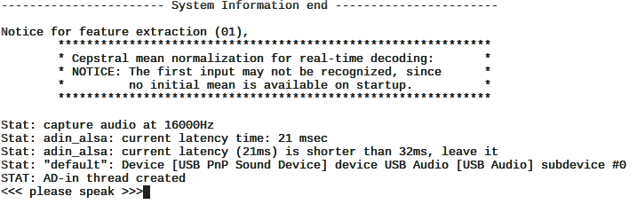
\includegraphics[width=0.8\textwidth]{../asset/image/text06-img009.png}
  \end{center}
  \textpageref{16}
\end{frame}

\begin{frame}
  \frametitle{辞書なしで比べる準備}
  \begin{itemize}
    \item 教科書16ページの果物から5つ選ぼう\\話す順番をメモしよう
    \item 同じ5語を、あとで辞書ありでも試そう
    \item 話しかけた言葉と認識結果を見比べよう
    \item 5個中、正しく認識した数を記録しよう
  \end{itemize}
  \textpageref{16}
\end{frame}

\begin{frame}
  \begin{exampleblock}{問題を解いてみよう}
    \begin{itemize}
      \item 教科書16ページ 問題7-7(1問)
    \end{itemize}
\end{exampleblock}
  \textpageref{16}
\end{frame}

\begin{frame}
  \frametitle{単語辞書}
  \begin{itemize}
    \item 認識させたい言葉を辞書にまとめる
    \item 候補を果物の名前にしぼって試そう
    \item 候補をしぼると認識結果はどう変わるかな？
  \end{itemize}
  \textpageref{17}
\end{frame}

\begin{frame}[fragile]
  \frametitle{単語辞書を使ってみる}
  \begin{itemize}
    \item 実行中のJuliusをCtrl+cで終了する
    \item 終了して入力待ちに戻ったことを確認する
  \end{itemize}
\begin{lstlisting}[title=ターミナル]
cd ~/07/
julius.sh kudamono.dic
\end{lstlisting}
  \begin{itemize}
    \item 辞書なしと同じ5語を同じ順番で話す
    \item 正しく認識した数を比べよう
  \end{itemize}
  \textpageref{17}
\end{frame}

\begin{frame}
  \begin{exampleblock}{問題を解いてみよう}
    \begin{itemize}
      \item 教科書17ページ 問題7-8(3問)
    \end{itemize}
\end{exampleblock}
  \textpageref{17}
\end{frame}

\begin{frame}
\frametitle{結果を見てみよう}
  \begin{center}
  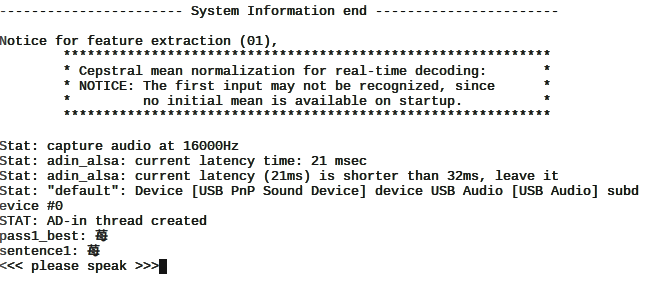
\includegraphics[width=0.8\textwidth]{../asset/image/julius_demo_strawberry.png} \\
  \end{center}
  話しかけた単語とターミナルに表示される単語は一致しているかな？
  \textpageref{17}
\end{frame}

\begin{frame}[fragile]
  \frametitle{単語辞書を作ってみよう -1}
  \begin{itemize}
    \item ラベル（コンピュータが使う名前）と読みを書く
    \item ラベルと読みは半角スペースで区切る
    \item 読みはひらがな。1語ずつ改行する
  \end{itemize}
\begin{lstlisting}[title=.yomiの例]
林檎 りんご
ブドウ ぶどう
みかん みかん
\end{lstlisting}
  \textpageref{18}
\end{frame}

\begin{frame}[fragile]
  \frametitle{単語辞書を作ってみよう -2}
  \begin{itemize}
    \item まず、果物を3語追加しよう
  \end{itemize}
\begin{lstlisting}[title=ターミナル]
cd ~/07/
mousepad kudamono.yomi
\end{lstlisting}
  \begin{itemize}
    \item 追加したらファイルを保存する
    \item 時間があれば、3語以上の独自辞書も作ろう\\例：動物や家電の辞書（jisho.yomi）
  \end{itemize}
  \textpageref{18}
\end{frame}

\begin{frame}
  \frametitle{単語辞書を作ってみよう -3}
  \begin{itemize}
    \item .yomi：人が編集しやすい、ラベルと読みの一覧
    \item .dic：Juliusが利用する形式の辞書
    \item convert\_yomi.shで.yomiを.dicに変換する
    \item 読みを変えたり語を追加したら、もう一度変換する
  \end{itemize}
  \textpageref{18}
\end{frame}

\begin{frame}[fragile]
  \frametitle{単語辞書を作ってみよう -4}
\begin{lstlisting}[title=ターミナル]
convert_yomi.sh kudamono.yomi > kudamono.dic
julius.sh kudamono.dic
\end{lstlisting}
  \begin{itemize}
    \item 「>」で変換結果を.dicファイルに保存する
    \item 終わるときはCtrl+c。終了を確認して次へ
    \item 独自辞書ならkudamonoをすべてjishoにする
  \end{itemize}
  \textpageref{18}
\end{frame}

\begin{frame}
  \begin{exampleblock}{問題を解いてみよう}
    \begin{itemize}
      \item 教科書19ページ 問題7-9(5問)\\最後の1問は時間があれば
    \end{itemize}
  \end{exampleblock}
  \textpageref{19}
\end{frame}

\begin{frame}
  \frametitle{HSPで\\Juliusの認識結果を使おう -1}
  \begin{figure}
    \includesvg[width=\linewidth]{../asset/image/JuliuswithHSP.svg}
  \end{figure}
  \textpageref{20}
\end{frame}

\begin{frame}
  \frametitle{HSPで使う4つのポイント}
  \begin{itemize}
    \item init\_julius：辞書を指定して音声認識を準備
    \item get\_word\_list：認識結果を受け取る
    \item words(cnt)：認識された言葉
    \item cm(cnt)：Juliusの自信の目安\\1に近いほど高いが、正解の確率ではない
  \end{itemize}
  \textpageref{20～21}
\end{frame}

\begin{frame}[fragile]
  \frametitle{HSPで\\Juliusの認識結果を使おう -2}
  \begin{lstlisting}[title=\textasciitilde/07/julius.hsp,label=julius.hsp-part1]
  #include "hsp3dish.as"
  #include "julius.as"

  redraw 0
  pos 0, 0
  mes "Loading Julius..."
  redraw 1

  init_julius "kudamono.dic" <#blue#;辞書ファイル読み込み#>

  sockidx = 0
  domain = "127.0.0.1"
  PORT = 10500
  \end{lstlisting}
  \textpageref{21}
\end{frame}

\begin{frame}[fragile]
  \frametitle{HSPで\\Juliusの認識結果を使おう -3}
  \begin{lstlisting}[title=\textasciitilde/07/julius.hsp,label=julius.hsp-part2]
  sockopen sockidx, domain, PORT

  if stat != 0 { <#blue#;エラー処理#>
    redraw 0
    mes "Error in opening socket"
    redraw 1
    wait 30
    stop
  }

  sdim words, 4096, 0
  ddim cm, 0
  \end{lstlisting}
  \textpageref{21}
\end{frame}

\begin{frame}[fragile]
  \frametitle{HSPで\\Juliusの認識結果を使おう -4}
  \begin{lstlisting}[title=\textasciitilde/07/julius.hsp,label=julius.hsp-part3,basicstyle=\scriptsize]
  repeat -1
    if is_recieved(sockidx) = 0 {
      get_word_list words, cm
      len =  "L1 " + length(words)
      repeat length(words)
        if cm(cnt) > 0.5 { <#blue#;単語信頼度が0.5より大きいとき#>
            ans =  "" + cnt + ": " + words(cnt) + " CM = " + cm(cnt)
        } <#blue#;words(cnt)が認識された文字、cm(cnt)が単語信頼度#>
      loop
    }
    redraw 0
    pos 0,0
    mes len
    mes ans
    redraw 1
    await 30
  loop
  \end{lstlisting}
  \textpageref{21}
\end{frame}

\begin{frame}
  \begin{exampleblock}{問題を解いてみよう}
    \begin{itemize}
      \item 教科書22ページ 問題7-10(2問)
    \end{itemize}
  \end{exampleblock}
  \textpageref{22}
\end{frame}

\begin{frame}
  \frametitle{困ったとき：Juliusとパス}
  \begin{itemize}
    \item 起動しないときは、ターミナルでstopjulius.sh\\を一度実行し、もう一度起動する
    \item HSPで指定するパスには「\texttt{\textasciitilde}」（チルダ）は使えない
    \item "kudamono.dic"は実行中のディレクトリから探す
    \item 別の場所なら、相対パスか絶対パスを使う
  \end{itemize}
  \textpageref{22}
\end{frame}

\begin{frame}[fragile]
  \frametitle{音声でLEDを動かす -1}
  \begin{lstlisting}[title=\textasciitilde/07/ledbyvoice.hsp,label=ledbyvoice.hsp-part1]
    #include "hsp3dish.as"
    #include "julius.as"

    redraw 0
    pos 0, 0
    mes "Loading Julius..."
    redraw 1

    init_julius "onoff.dic" <#blue#;辞書を読み込む#>

    sockidx = 0
    domain = "127.0.0.1"
    PORT = 10500
  \end{lstlisting}
  \textpageref{23}
\end{frame}

\begin{frame}[fragile]
  \frametitle{音声でLEDを動かす -2}
  \begin{lstlisting}[title=\textasciitilde/07/ledbyvoice.hsp,label=ledbyvoice.hsp-part2]
    sockopen sockidx, domain, PORT

    if stat != 0 {
      redraw 0
      mes "Error in opening socket"
      redraw 1
      wait 30
      stop
    }

    sdim words, 4096, 0
    ddim cm, 0
  \end{lstlisting}
  \textpageref{23}
\end{frame}

\begin{frame}[fragile]
  \frametitle{音声でLEDを動かす -3}
  \vspace{0.45cm}
  \begin{lstlisting}[title=\textasciitilde/07/ledbyvoice.hsp,label=ledbyvoice.hsp-part3,basicstyle=\scriptsize]
  repeat -1
    if is_recieved(sockidx) = 0 {
      get_word_list words, cm
      repeat length(words)
        if cm(cnt) > 0.7 {                <#blue#;単語信頼度が0.7より大きいとき#>
          if words(cnt) = "ON" {          <#blue#;認識された文字がONのとき#>
            gpio 17, 1                    <#blue#;GPIO17のLEDを光らせる#>
          }else : if words(cnt) = "OFF" { <#blue#;認識された文字がOFFのとき#>
            gpio 17, 0                    <#blue#;GPIO17のLEDを消す#>
          }
        }
      loop
    }
    redraw 0
    pos 0,0
    mes "話しかけてLEDのONとOFFをしよう"
    redraw 1
    await 30
  loop
  \end{lstlisting}
  \textpageref{23}
\end{frame}

\begin{frame}[fragile]
  \frametitle{言葉とLEDの対応}
\begin{lstlisting}[title=onoff.yomi]
ON おん
OFF おふ
\end{lstlisting}
  \begin{itemize}
    \item 左がラベル、右が読み方
    \item words(cnt)がONなら点灯、OFFなら消灯
    \item cm(cnt) > 0.7のときだけ結果を使う
  \end{itemize}
  \textpageref{24}
\end{frame}

\begin{frame}
  \begin{exampleblock}{問題を解いてみよう}
    \begin{itemize}
      \item 教科書24ページ 問題7-11(5問)\\最後の1問は時間があれば
    \end{itemize}
  \end{exampleblock}
  \textpageref{24}
\end{frame}

\begin{frame}
  \frametitle{しきい値を比べてみよう}
  \begin{itemize}
    \item cmのしきい値を0.3、0.7、0.9に変えて試す
    \item それぞれで「ON」「OFF」と、辞書にない言葉\\（例：「こんにちは」）を話しかける
    \item 反応のしやすさと、関係のない言葉への反応を比べる
  \end{itemize}
  \textpageref{24}
\end{frame}

\begin{frame}[fragile]
  \frametitle{時間があれば：\\読み方を変えよう}
  \begin{itemize}
    \item ラベルON / OFFはそのまま、読みを変える
  \end{itemize}
\begin{lstlisting}[title=onoff.yomi]
ON つける
OFF けす
\end{lstlisting}
  \begin{itemize}
    \item 保存後は辞書を作り直して、HSPを再実行する
  \end{itemize}
\begin{lstlisting}[title=ターミナル]
convert_yomi.sh onoff.yomi > onoff.dic
\end{lstlisting}
  \textpageref{24}
\end{frame}

\begin{frame}
  \frametitle{宿題}
  \begin{itemize}
    \item 教科書25ページの5問から好きな問題を1つ以上
    \item キー入力で数字を読み上げる
    \item 画像をクリックして名前を読み上げる
    \item 声で文字の色や表示する画像を変える
  \end{itemize}
  \textpageref{25}
\end{frame}

\begin{frame}
  \frametitle{数を認識させてみよう（発展）}
  \begin{itemize}
    \item 言葉を組み合わせるルールを「文法」で決める
    \item 例：「ひゃく」＋「にじゅう」＋「さん」\\→「ひゃくにじゅうさん」
    \item 数を一つずつ単語として登録する手間を減らせる
    \item 7には「なな」「しち」のような読み方もある
    \item 興味があれば、先生に聞いてみよう
  \end{itemize}
  \textpageref{26}
\end{frame}

\begin{frame}
  \centering
  実験
\end{frame}

\begin{frame}
  \frametitle{音声でできることを考えよう}
  \begin{itemize}
    \item 例えば…
    \begin{itemize}
      \item ボタンを押すと話してくれる
      \item 気温や湿度を教えてくれる
      \item 指示した色のLEDを光らせてくれる
      \item 時刻を聞くと時刻を話してくれる
      \item 日付を聞くと日付を話してくれる
    \end{itemize}
    \item 例を参考に何が作れるかを自分で考えてみよう
  \end{itemize}
\end{frame}

\begin{frame}
  \frametitle{作りたいものを考えよう}
  \begin{itemize}
    \item Open JTalkやJuliusを使って作りたいものを考えてみよう(5-10分)
    \item チームのみんなで作りたいものを発表してみよう、一緒に考えてみよう(5-10分)
    \begin{itemize}
      \item むずかしさはどれくらいだろう
      \item どうやって作ればいいだろう
    \end{itemize}
  \end{itemize}
\end{frame}

\begin{frame}
  \frametitle{手順}
  \begin{itemize}
    \item 演習用のフォルダを作る
    \item 使う.hsp、.yomi、.dicをコピーする
    \item 声音のフォルダも中身ごとコピーする\\htsvoice-tohoku-f01の名前と構造を保とう
    \item プログラムからの相対パスが合うか確認する
    \item プログラムを書き換えたり、新しく作ったりしよう
  \end{itemize}
\end{frame}

\begin{frame}
  \frametitle{できたものをチームのみんなに教えよう}
  \begin{itemize}
    \item どんなものを作ったか
    \item 工夫したところはどこか
    \item どうしてその作品を作ったか
  \end{itemize}
  実際に作品を動かしてみんなに見せてみよう！
\end{frame}

\end{document}
